%=========================================================================

\chapter{Úvod}
Žijeme v době kdy se internet stal nedílnou součástí každodenního života a s internetem už nepracují
pouze klasické počítače, ale do popředí se také dostávají mobilní zařízení, které meziročně
zaznaménavají více než $50\%$ nárůst. Dalším druhem zařízení jež se začínají připojovat
jsou vestavěné systémy patřící do trendu nazývaného internet věcí.
S rychlostí jakou přibývají zařízení vyžadující přístup k internetu ale i s rozšiřováním internetu
do zemí internetem nedotčených se neustále zvyšují požadavky na rychlost, se kterou data prochází počítačovými
sítěmi a z toho vyplívající požadavky na rychlost zpracování síťového provozu a to zejména na zařízeních
starajících se o řízení internetového provozu na páteřních linkách počítačových sítí. Mezi tyto
zařízení lze zařadit směrovače (routery), které řídí datové toky mezi jednotlivými sítěmi,
rozbočovače (switche) starající se o řízení toků dat uvnitř autonomních sítí a
systémy pro detekci (IDS\footnote{Intrusion detection system}) a prevenci (IPS\footnote{Intrusion prevention system})
síťových útoků, které analyzují obsah každého paketu, který sítí prochází.
Páteřní spoje v době psaní této práce dosahují rychlostí v řádech gigabitů
za sekundu a z toho vyplívají požadavky na rychlost zpracování síťových dat. Při těchto rychlostech
však tradiční procesory stihnou vykonat pouze desítky instrukcí, které nestačí na provedení včech potřebných
operací. Nicméné je důležité aby stejné rychlosti zpracování dosahovaly všechna zařízení na páteřních spojích,
protože v počítačová sít je pouze tak rychlá, jak rychlá je její nejpomalejší část, tzv. úzké hrdlo.
Z těchto vlastností vycházejí požadavky na stále efektivnější algoritmy zpracovávající časově kritické operace,
jejichž rozbor je součástí této práce. Z těchto operací jsou vybrány a rozvedeny operace prohledávání vstupních
dat na přítomnost definovaných slov pomocí vyhledávání řetězců a  hledání regulárních výrazů pro hledání signatur
útoků v počítačovém provozu, analýza a extrakce hlaviček paketů - operace používané napříč téměř všemi časově kritickými operacemi a klasifikace paketů, speciálně pak jednodimenzionální klasifikace podle cílové IP adresy,
hledání nejdelšího shodného prefixu, jež je využíváno pro prohledávání směrovací tabulek směrovačů pro
nalezení takové cesty počítačovou sítí, která bude nejhodnější.

Přínosem této knihovny je vlastní implementace zmíněných časově kritických operací, která bude
využita výkumnou skupinou ANT na Fakultě Informačních technologií Vysokého učení technického v Brně
pro ??????????? a také může sloužit jako vzor pro hardwarovou akceleraci procházení a vyhledávání ve
zmíněných operací buď syntézou kódu do programovatelných hradlových polí FPGA\footnote{Field Programmable Gate Array}
nebo pro návrh samostatnéhých integrovanéhých obvodů ASIC\footnote{Application Specific Integrated Circuit}.
Pro knihovnu je navržen a implementován obecný princip vláknového zpracování použitelný pro všechny
zmíněné operace, který umožňuje řetězit požadavky na zpracování do vyrovnávacích pamětí a jednotlivé operace
provádět plynule za sebou bez nutnosti zasahovat do datových struktur nebo toku řízení.

V kapitole \ref{chapter:theoretical} jsou popsány síťové modely a vrstvy těchto modelů,
nad nimiž jsou operace této knihovny implementovány, dále jsou popsány časově kritické operace prováděné
prvky v počítačových sítích. Kapitola \ref{chapter:api} popisuje návrh veřejného rozhraní vytvořené knihovny
pro operace zmíněné v kapitole \ref{chapter:theoretical}, způsoby použití potéto knihovny a možnosti rozšíření
o další časově kritické operace. V kapitole \ref{chapter:results} jsou vizualizovány a diskutovány
výsledky, jež se podařilo dosáhnout v implementaci této knihovny a to na dvou hlavních platformách, Intel a ARM.
Kapitola \ref{chapter:conclusion} shrnuje dosažené výsledky a nastiňuje další možný vývoj této knihovny
a to jak z hlediska rozšiřování repertoáru implementovaných operací tak i z pohledu dalších optimalizací
a testování v různých scénářích při reálném používání knihovny.

\paragraph{Co zmínit}
- všchny prvky musí pracovat na stejných rychlostech
- zvyšuje se rychlost -> nutná optimalizace, fpga
- požadavky na monitorování a blokování
- ipv4, ipv6, velikost adresového prostoru
- pomalé procesory -> směr fpga, jak je na to knihovna přpravena
- koncept multithreadingu
- hlavní síťové prvky
- páteřní sítě
- pakety
- půlstrana motivace proč je to důležité
- přínos knihovny a operace
- vlákna - plná fronta nebo timeout pro spuštění

\chapter{Teoretický rozbor}\label{chapter:theoretical}

\paragraph{Co zmínit}
- složitost síťového provozu, proto vrstvy
- něco o kritických operacích
- proč jsou důležité
- popsat další kapitoly

\section{Síťové modely}
Zpracování dat síťového provozu je rozděleno do několika úrovní. Tyto úrovně jsou popsány síťovými modely.
Základním modelem je ISO/OSI, který slouží pro abstraktní rozdělení operací zpracování síťových dat a jeho použití je
pouze pro akademické účely. V reálných počítačových sítích pak dominuje model TCP/IP, který má oproti
ISO/OSI modelu menší počet vrstev. Modelu ISO/OSI je rozdělen na sedm vrstev. V pořadí od nejnižší úrovně to
jsou vrstvy fyzická, linková, síťová, transportní, relační, prezentační a aplikační. Pro tuto práci jsou
podstatné pouze první čtyři vrsty. Ty jsou detailněji popsány v kapitolách \ref{layers:physical},
\ref{layers:link}, \ref{layers:network} a \ref{layers:transport}. Na obrázku \ref{fig:layers} je
znázorněn průchod dat jednotlivými vrstvamy modelu ISO/OSI. Jak je z obrázku patrné tak ne všechny síťové
zařízení pracují na stejných vrstvách.

\begin{figure}[!htb]
	\centering
	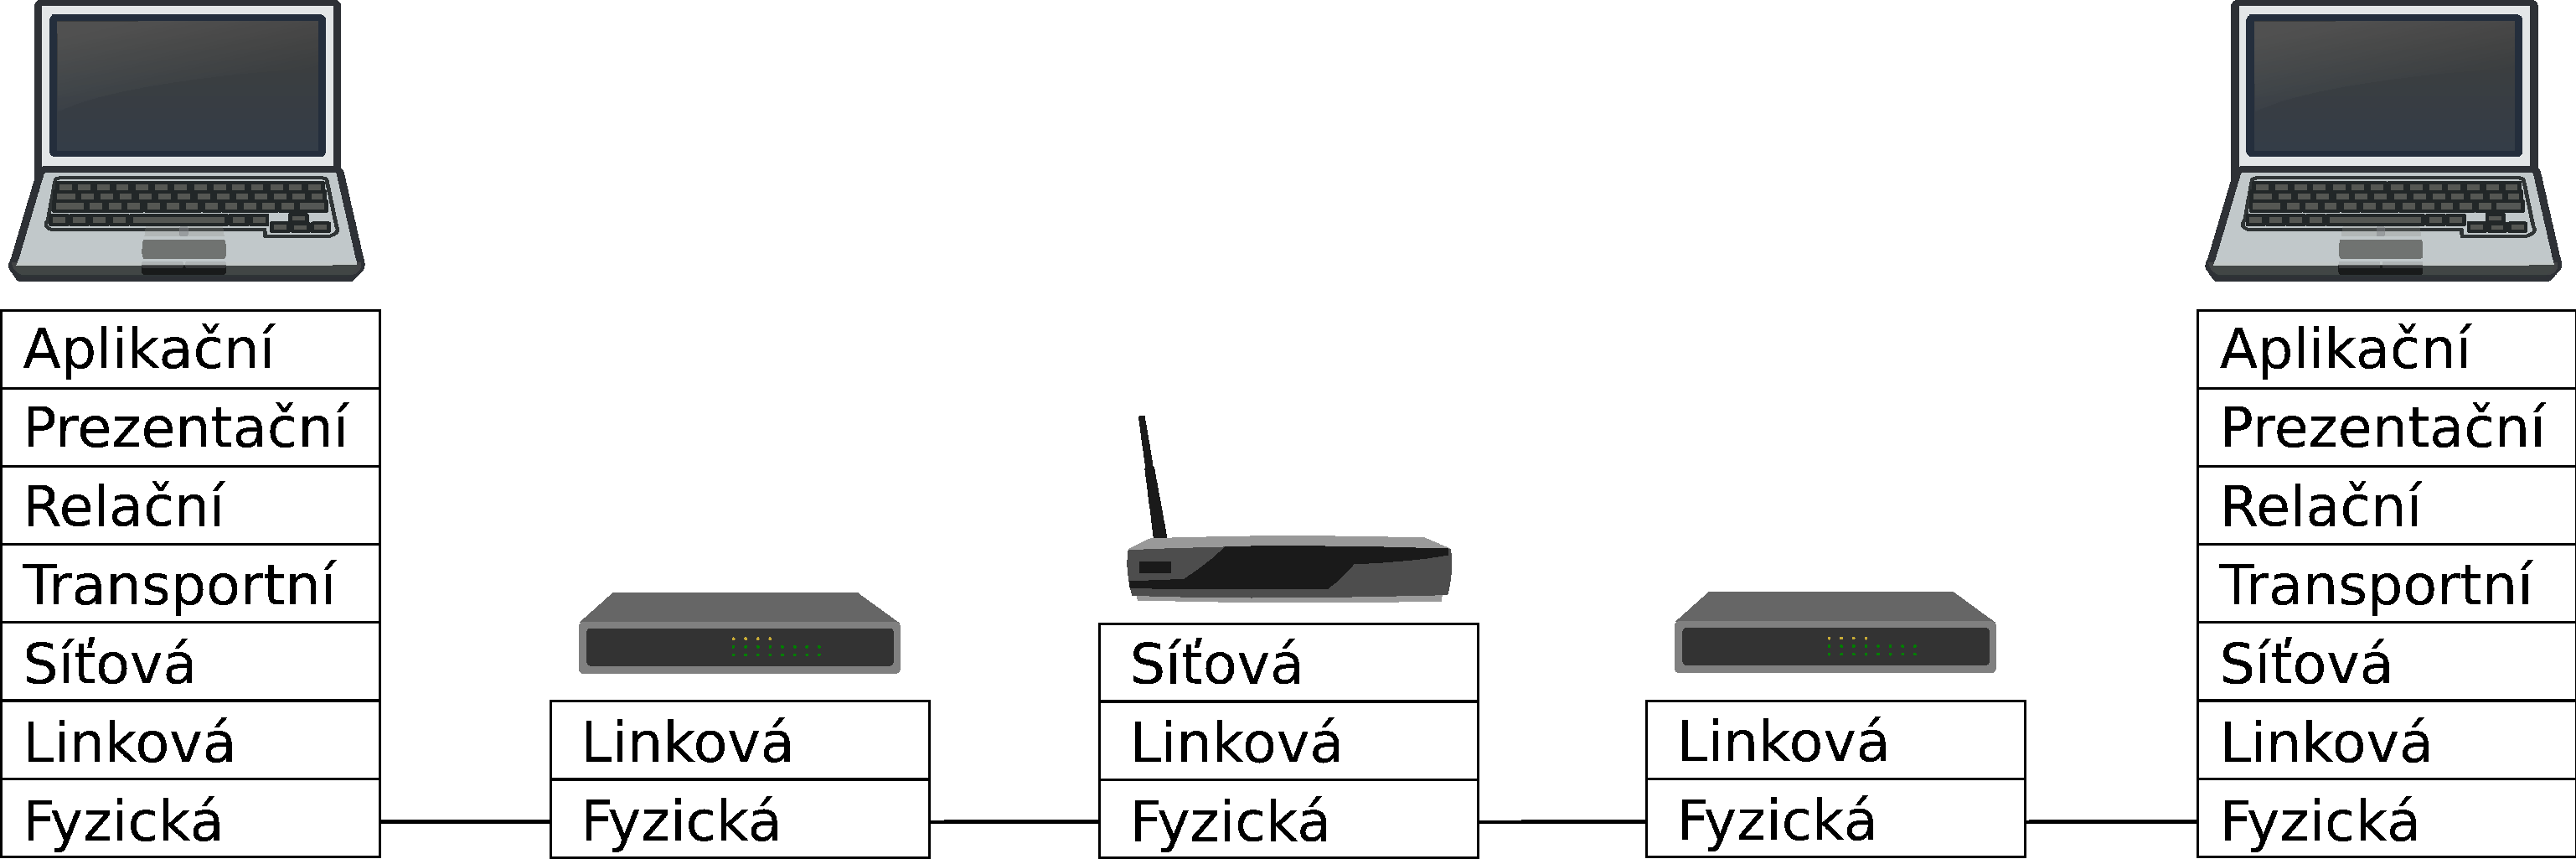
\includegraphics[scale=.25]{fig/layers.pdf}
	\caption{Znázornění průchodu dat počítačovou sítí v modelu ISO/OSI}
\end{figure}\label{fig:layers}

\subsection{Fyzická vrstva / Vrstva síťového rozhraní}\label{layers:physical}
Nejnižší vrstva ISO/OSI modelu pracuje s daty na úrovni bitů a stará se o
jejich přenos po přenosovém médiu. Protokoly této vrstvy definují signály, které reprezentují data
a tudíž jde o protokoly implementované již v hardware síťových zařízení.

\subsection{Linková vrstva}\label{layers:link}
Linková vrstva je druhá nejnižší ISO/OSI modelu. Tato vrstva se stará o datovou komunikaci
obecně mezi několika uzly, které jsou přímo spojeny. Spojení může být jak fyzickým vodičem tak i
bezdrátovou technologií. Nejrozšířenější technologií pro fyzické spoje je Ethernet IEEE 802.3, pro bezdrátové spoje
je to standard IEEE 802.11. Datová jednotka na linkové vrstvě se nazývá rámec a nese v sobě kromě
zapouzdřených dat vyšších vrstev také informace o kontrolním součtu dat a adresování pomocí MAC adres.
MAC adresa je adresa fyzického zařízení, které pracuje na této vrstvě.
Adresování MAC adresou slouží pro identifikaci zařízení, které se nacházejí ve stejné počítačové síti
a za hranici této sítě se již používá IP adresace, které je vysvětleno v necházející kapitole \ref{layers:network}
Síťová zařizení pracující na této vrstvě se nazývaji switche. Úkolem switchů je zjistit MAC adresu cílové stanice a přeposlat je portem, který vede k tomuto zařízení.

\subsection{Síťová vrstva}\label{layers:network}
Na této vrstvě probíhá komunikace za využití IP adres. Prvky používané na této vrstvě jsou nazývaný routery.
Účelem těcho zařízení je směrování paketů procházejících sítí. K tomu využívají směrovací tabulku.
Právě pro problém vyhledání nejdelšího shodného prefixu v routovací tabulce směrovače jsou v této knihovně
implementovány dva algoritmy, \texttt{Binary search on prefix length} \ref{} a \texttt{TreeBitmap} \ref{}.
Datové struktury jsou pojmenované pakety. Pakety obsahují imformace o datovém toku a také zrojové a cílové adresy (IPv4 nebo IPv6) právě tohoto paketu.

\subsection{Transportní vrstva}\label{layers:transport}
Transportní vrstva pracuje s datovou strukturou zvanou segmenty.
Obsahují informace jako je kontrolní součet pro zjištění integrity dat,
pořadové číslo rámce pro spojení dat, která byla na cestě k cíli rozdělena na více částí a také obsahuje čísla portů
pro určení uživatelských aplikací, která data odeslala a která je na druhém konci má přijmout.
Na transportní vrstvě se používají dva protokoly a to TCP a UDP. UDP má nižší režii ale zase je nespolihvé.
To znamená že paket do cílového zařízení nemusí vůbec dorazit a nebo můžé dorazit v jiném pořadí než byl ze
zdrojové stanice odeslán. Situace ve kterých pozitiva jako nižší režie přebyjí zápory je hlavně přenos dat v
reálném čase. To je například streamování videa, přenost hlasu technologie VoIP a přenos informací do online her.
Spolehlivý protokol TCPzaručuje, že všechna data budou přenesena a v cílové stanici se seřadí do
stejné posloupnosti v jaké byla odeslána. Důvodem proč se data mohou rozdělit je nestabilní cesta,
po které jsou data v síti směrována. Při přenosu jednoho toku dat se může stát že se jedna cesta po které se
již poslala část dat stane nedostupnout a místo toho se data začnou směrovat přes jiná zařízení.

Zpracování dat na úrovni transportní vrstvy a všech vyšších vrstev není implementováno na síťových
zařízeních starajících se přenost dat po síti. Jediná zařízení, které implementují zpracování
dat těchto vrstev jsou koncová zařízení.

\section{Časově kritické operace}
Pod pojmem časově kritické operace se rozumí takové operace, které je typicky nutné provádět
na více síťových zařízeních. Těmito zařizeními mouhou být routery, switche firewally a také systémy
oddělené od řízení síťového provozu jako například sondy pouze monitorující síťový provoz
nebo analyzátory, které mohou hledat signatury útoků v datových tocích.
Mezi časově kritické operace rozebrané v této práci patří klasifikace paketů a velký důraz je kladen specielně na
jednodimenziální klasifikaci dle cílové IP adresy, vyhledávání nejdelšího shodného prefixu.
Tato operace je využívána pro směrování na routerech.
Dalšími z operací je hledání podřetězců a hledání regulárních výrazů. Poslední dvě zmíněné operace
slouží především pro detekci útoků v systémech IDS (intrusion detection system) a pro prevenci útoků v systémech
IPS (intrusion prevention system).

\paragraph{Co zmínit}
- co jsou tyto operace
- na čem staví algoritmy
- proč jsou kritické
- zvyšování požadavků
- rychlost zpracování
- počet instrukcí při  různých rychlostech

\subsection{Hledání nejdelšího společného prefixu - Longest prefix matching}
Problém hledání nejdelšího shodného prefixu se rozumí klasifikace paketů dle jejich cílové IP adresy,
která může být jak verze 4, tak verze 6.

Tato operace je základním stavebním kamenem v počítačových sítích a bez ní by bylo téměř nemožné dosahovat
efektivity jaké se dosahuje teď. Hledání nejdelšího shodného prefixu je operace, která se provádí
na síťových prvcích zvaných směrovače. Tyto prvky jsou umístěny na každém rozhraní dvou a více
počítačových sítích. Jejich cílem je nalézt nejvhodnější cestu, kterou směrovat příchozí paket.
Struktura reprezentující uložené směrovací informace se nazývá routovací tabulka. Tato tabulka ukládá
informace o dostupných sítích (jejich prefixech), délce tohoto prefixu a rozhraní, kterým se lze
do odpovídající počítačové sítě dostat. S velkým rozmachem počíačových sítí v poslední dekádě
dochází k velkému nárustu routovací informací a proto se tímto směrem začal ubírat akademický výzkum.
Pro zmenšení routovacích tabulek byl navržen takzvaný supernetting, který sdružuje sítě se stejným
prefixem o jiných délkách a stejnou cestou do jedné sítě. Tím je dosaženo zmenšení routovacích tabulek,
nicméně i tak je potřeba v routovacích tabulkách vyhledávat efektivně.

Nejdelší shodný prefix se zapisuje jako $1001*$ a tento zápis reprezentuje všechny IP adresy,
které v binární podobě začínají právě na hodnotou $1001$. Nicméně v routovací tabulce
může být uložen i prefix $10010*$, který sdílí první čtyři bity své adresy s výše uvedeným příkladem,
a přípaďě, že přijde paket začínající hodnotou $10010$ je z pohledu směrování vyhodnotit prefix B jako
nejdelší a poté paket správně směrovat. V případě $10011$ je však nejdelším shodným prefixem pravidlo A
a tudíž nesmí dojít k vyhodnocení prefixu B jako nejdelšího. Z toho důvodu je nutné ve směrovací tabulce
uchovávat i informace o délce prefixu. Tato informace poté slouží pro rozhodnutí, jaký pravidlo
routovací tabulky má nejdelší shodný prefix. Délká prefixu může nabývat hodnot $1-32$ pro adresy typu
IPv4 a $1-128$ pro adresy typu IPv6. Z výše uvedených tvrzení je zřejmé, že pro každý typ
IP adres musí existovat samostatná, oddělená routovací tabulka, jinak by mohlo docházet k nevalidním
vyhodnocení nejdelšího shodného prefixu mezi IPv4 a IPv6 adresami. Jako příklad může sloužit následující
situace

100* 3 R1 IPv4\
100* 3 R7 IPv6\

Teoreticky by bylo možné ukládat různé typy prefixů do stejných datových struktur pro algoritmus
Binary search on prefix length, nicméně by bylo nutné explicitně rozlišovat o jaký typ IP adresy se
jedná a to by mělo negativní vliv na rychlost vyhledávání. To je právě kritický paramter, který
se snažíme minimalizovat.

Pro hledání nejdelšího shodného prefixu existuje velké množství algortimů, které jsou popsány v \cite{}
Většina z nich je založena na procházení stromové struktury. Každý algoritmus má jiné paměťové nároky
a dosahuje jiných rychlostí. Je nutné zvolit kompromis mezi rychlostí a paměťovou náročností.
V připadě že jde o implementaci na architektuře FPGA důraz bude pravděpodobně kladen na paměťovou náročnost
a to z důvodu, že tyto čipy mají specializované paměti. Tady bych zmínil asociativní paměť, kterou
lze přímo použít pro vyhledávání. Na architekturách vycházejících z x86 je naopak kladen důraz
na rychlost zpracování z důvodů obecných procesorů, které nejsou specializovány na tyto operace
ale naopak zase disponují standardními paměťmy, které jsou lehce škálovatelné a dosahují kapacit
řádově převyšující nároky jednotlivých algoritmů.

Algoritmy rozehrané v této kapitole vycházejí z obecně n-árního stromu,
což je rozšíření binárního stromu na více než dva potomky. Těmito algoritmy jsou
\texttt{Binary search on prefix length}, jehož data jsou uložena v binárním stromu, ale pro vyhledávání
je využito výhod hašovací tabulky, a \texttt{TreeBitmap}, který je n-árním stromem, kde n je volitelné.
Dosažené výsledky pro různé n jsou vizualizovány v kapitole \ref{}.

První algoritmus hledání nejdelšího shodného prefixu byl založen na naivním procházení lineárního
seznamu a byl publikován v knížce X v roce Z. Jak si čtenář může dovtípit do vyhledání
byla závislá na počtu uložených prefixů a její časová složitost byla $O(N)$.
Algoritmy popsané a implementované v rámci této práce se minimalizují dobu vyhledávání v závislosti
na počtu prefixů v routovací tabulce. V případě binary search on prefix length je tato závislost
omezená vlastnostmi hašovací funkce. Pokud je zvolena špatná hašovací funkce bude docházet ke kolizím
a v případě nefunkční hašovací funkce (generuje stejný výsledky pro řůzné prefixy)
ořezán na prosté procházení lineárního seznamu.


\paragraph{Co zmínit}
- jaké jsou známené algoritmy
- hašovací funkce
- výhody/nevýhody těchto algoritmů
- první algoritmus
- směrovací protokoly
- co obsahuje směrovací tabulka
- jedna adresa může odpovídat více záznamům
- příklad směrovací tabulky s stejnými adresami a různou délkou
- délka je počet bitů adresy sítě
- umísťění zařízení má vliv na velikost tabulky - nějaký příklad?
- sekvenční vyhledávání v seznamu
- TCAM, asociativní paměť?
- trie struktura?
- binární trie
- multibitový trie
- klíč je určen implicitně pozicí ve stromu a ne explicitně


\subsubsection{TreeBitmap}

Struktura pro uložení prefixu se skládá z položek interní bitmapy, externí bitmapy, ukazatele na potomky
a ukazatele na pravidla. Interní bitmapa zahrnuje všechny všechny prefixy,
které je možné vyjádřit na N bitech střídy. Jako příklad může posloužit velikost střidy 2 bity.
Proto je nutné uložit všechny tyto kombinace: $0*$, $1*$, $00*$, $01*$, $10*$ a $11*$.
Z toho lze odvodit vzorec pro počet bitů nutných pro reprezentaci všeh možný stříd.
$2^{N + 1}$ kde N je velikost střídy. Velikost externí bitmapy lze vyjádřit vzorcem $2^N$ kde N je velikost střídy.

Interní bitmapa slouží pro zjištění, kolik pravidel existuje v tomto uzlu.
To se zjistí zavolání funkce \texttt{ones(internal-bitmap, end)}. kde end pozice,
která odpovídá části prefixu o délce střídy.
To znamená že pokud po vykousnutí střídy z prefixu dostaneme bity
$11$ pozice end bude stanovena na decimální reprezentaci tohoto čísla, v tomto případě $3$.
Následuje zjištění, zda se na dané pozici interní bitmapy vykytuje jednička nebo nula.
V případě, že je tam nula se neděje nic a algoritmus pokračuje zjišťováním, zda existuje
cesta stromem dál z externí bitmapy jak je vysvětleno v následujícím odstavci.

Pokud je tam jednička tak algoritmus spočítá funkci ones na interní bitmapě a uloží si vypočítanou
hodnotu. Dále si také uloží odkaz do tabulky pravidel.

Pokud tam není jednička, tak se postupně odebírají méně významné bity vykousnuté v prefixu a v cyklu se provádí
zjišťování zda je tam jednička nebo ne. Tento cyklus je ukončen v případě, že se narazí na nultou pozici
nebo je nalezena jednička.

V přípaďě že již neexisuje další cesta stromem je algoritmus vyhledávání ukončen a jako výsledek
je navrácena hodnota uložená ukazateli na nejlepší pravidla s index, který je uložen také.

Externí bitmapa slouží pro zjíštění, zda existuje cesta ve stromu, která odpovídá vyzobnutému prefixu.
Index do pole následovníků je vypočítán jako \texttt{ones(external-bitmap, end)}. V případě,
že pro vyzobnuté bity neexistuje následovník je navráceno pravidlo, které bylo zjištěno z interní bitmapy.

Funkce \texttt{ones(bitmap, end)} spočítá všechny bity, které jsou nastaveny na jedničku v rozmezí $<0, end)$.
Toto je implementuje jako bitová operace \texttt{AND} a maskou, která reprezentuje právě počet pozic, které se
mají vypočítat. Samotné zjištění počtu jedniček lze řešit několika způsoby, v implementaci této knihovny
je zvoleno volání vestavěné funkce překladače \texttt{popcount}, které se při překladu převede na nejefektivnější
instrukce cílové platformy.

Algoritmus v pseudokódu je možné vidět v \ref{alg:treebitmap}.

Příklad bitmap pro uložení prefixů:

\begin{table}
	\center
	\label{tab:tbm-internal}
    \begin{tabular}{|l||c|c|c|c|c|c|c|}
    \hline
    Prefix & $*$ & $0*$ & $1*$ & $00*$ & $01*$ & $10*$ & $11*$ \\ \hline
    Pravidlo & 0 & 0  & 1  & 0   & 0   & 1   & 1   \\ \hline
    \end{tabular}
    \caption{Příklad interní bitmapy}
\end{table}

\begin{table}
	\center
	\label{tab:tbm-external}
    \begin{tabular}{|l||c|c|c|c|}
    \hline
    Prefix & $00*$ & $01*$ & $10*$ & $11*$ \\ \hline
    Pravidlo & 1 & 0 & 1 & 0 \\ \hline
    \end{tabular}
    \caption{Příklad externí bitmapy}
\end{table}

Treebitmap je šetrný k paměti a alokuje si pouze tolik prvků pole ať už pro uložení pravidel
nebo pro uložení následovník kolik jich je opravdu potřeba.

Z \cite{tbm} vyplívá, že je vhodné nastavit velikost střídy v rozmezí 2 - 8 bitů. Což je také rozmezí,
na které je sousředěna a otestována implementace TreeBitmap v této knihovně. Experimentálně bylo zjišténo,
že tato implementace je funkční až do velikost střídy 13bitů.

\begin{algorithm}[H]
	\label{alg:treebitmap}
	\KwData{tbm-root, ip, ip-length}
	\KwResult{routing rule}
	node $\leftarrow$ tbm-root\;
	position $\leftarrow$ 0\;
	\Repeat{BIT(parent.external, bits)}
	{
		bits $\leftarrow$ get-stride-bits(ip, position, prefix-length)\;
		position $\leftarrow$ position + STRIDE\;

		\If{isRule(node.internal, bits)}
		{
			longest-match = node\;
		}

		index $\leftarrow$ ones(node.external, bits)\;
		parent $\leftarrow$ node\;
		node $\leftarrow$ node.external[index]\;
	}
	\Return longest-match\;
	\caption{Hledání nejdelšího shodného prefixu algoritmem TreeBitmap}
\end{algorithm}

\paragraph{Co zmínit}
- procházení interních a externích bitmap, struktura interní a externí bitmapy
- alokace všech násldovníků a pravidel na jednou v jednom místě
- funkce jedniček

\subsubsection{Binary search on prefix length}
Algorimus binary search on prefix length je založen jak již název napovídá na binárním vyhledávání.
Binaární vyhledávání jiný název pro půlení intervalů. Vyhledávání půlením intervalů
se ve své první iteraci pokusí vyhledat shodný prefix celé délky, tedy 32 bitů pro IP adresu
verze protoklou IPv4 a 128 bitů pro IP verze 6.

Mějme směrovací tabulku obsahující tyto informace:

\begin{table}[!htbp]
	\center
    \begin{tabular}{|l|l|l|}
    \hline
    Prefix        & Délka prefixu & Pravidlo \\ \hline
    147.228.0.0   & 14            & P1       \\ \hline
    147.228.128.0 & 17            & P2       \\ \hline
    \end{tabular}
    \caption{Příklad směrovací tabulky}
\end{table}

Vyhledávání směrovací cesty pro adresu 147.229.128.54 bude procházet následujícími kroky

\begin{table}[!htbp]
	\center
    \begin{tabular}{|l|l|l|l|}
    \hline
    Prefix & Délka prefixu  & Změna prefixu & Průběžný výsledek \\ \hline
    147.228.128.54 & 32 & 16 & Nenalezeno, zmenšit délku \\ \hline
    147.228.0.0 & 16 & 8 & Nenalezeno, zvětšit délku \\ \hline
    147.228.128.0 & 24 & 4 & Nenalezeno, zmenšit délku \\ \hline
    147.228.128.0 & 20 & 2 & Nenalezeno, zmenšit délku \\ \hline
    147.228.128.0 & 18 & 1 & Nenalezeno, zmenšit délku \\ \hline
    147.228.128.0 & 17 & 0 & Nalezeno, vrátit P2 \\ \hline
    \end{tabular}
    \caption{Příklad vyhledání nejdelšího shodného prefixu}
\end{table}

Operace vyhledání nejdelšího prefixu při využití algoritmu binary search on prefix length má časovou
složitost $\log{2}{N}$, kde \texttt{N} je počet bitů adresy. V případě IPv4 adresy je to 32 bitů a pro IPv6
adresu je to 128 bitů. Z principu algoritmu vyplívá, že nejhorší výsledky z časového hlediska bude dosahovat
při shodě prefixu, který byl zadán s lichou délkou. V tomto případě bude nutné projít všemy kroky.
Počet kroků v případě IPv4 bude 5 a v případě IPv6 adresy to pak bude 7.
Zde je vidět že i v připadě čtyřikrát delší adresy se počet kroků pro vyhledání prefixu zvedne pouze o dva,
což neplatí pro algoritmus TreeBitmap, který musí projít v nejhorším případě až čtyřikrát více
uzlů aby nalezl odpovídající prefix.
\cite{bspl}

\begin{algorithm}
	\KwData{bspl-root, hash-table, ip, ip-length}
	\KwResult{routing rule}
	prefix-length $\leftarrow$ ip-length\;
	prefix-change $\leftarrow$ ip-length\;
	\Repeat{prefix-change $>$ 0}
	{
		bits $\leftarrow$ get-prefix-bits(ip, prefix-length)\;
		item $\leftarrow$ hast-table.get(bits)\;
		prefix-change $\leftarrow$ prefix-change $\gg$ 1\;

		\If{item == NULL}{prefix-length $\leftarrow$ prefix-length - prefix-change\;}
		\ElseIf{item.type == PREFIX}{prefix-length $\leftarrow$ prefix-length + prefix-change\;}
		\lElse{break}
	}
	\lIf{item == NULL}{\Return bspl-root.default-rule}
	\caption{Hledání nejdelšího shodného prefixu algoritmem Binary search on prefix length}
\end{algorithm}

\paragraph{Co zmínit}
- leaf-pushing?

\subsection{Hledání řetězců}
V počítačových sítích je často vyžadováno hledání řetězců v síťovém provozu ať už z důvodu monitorování
nebo blokování provozu, který obsahuje určité řetězce. Blokování může probíhat na úrovni obsahu, například
blokování určitých webových stránek ať už z důvodů rodičovské kontroly nebo například omezení provozu
netýkajícího se výuky ve školních sítích. Nebo může jít o blokování určitého druhu síťového provozu,
který obsahuje nedovolené nebo podezřelé signatury. Pokud se vzdálí ze síťového provozu tak
důvodem pro vznik těchto algoritmů je hledání v textových datech. I z tohoto důvodu vznikl
algoritmus Aho-Corasick, který je v této knihovně implementován a původně byl navržen
právě pro hledání klíčových slov v odborných publikacích.

Pro hledání řetězců je implementován algoritmus autorů Aho a Corasicové. Tento algoritmus používá pro zjištění shody s podřetězcem konceptu konečného automatu. Při každé iteraci algoritmu se provede přechod o jeden znak.

Algoritmus procházení vstupních dat je rozepsán v \ref{alg:aho} a vychází z \cite{aho}.

\begin{algorithm}
	\KwData{start-state, text}
	\KwResult{keyword}
	state = start-state\;
	\For{position $\leftarrow$ 0 \KwTo text.length}
	{
		\lWhile{goto(state, text[position]) == FAIL}{state $\leftarrow$ state.failure}
		\lIf{state.isMatch}{\Return state.keyword}
	}
	\Return NOT-MATCH\;
	\caption{Algoritmus procházení textu a hledání podřetězců}
\end{algorithm}\label{alg:aho}

Při chybě alokace se smaže celá struktura konečeného automatu, neexistuje předpoklad na dynamické přidávání pravidel za běhu programu

\subsection{Hledání regulárních výrazů}

Regulární výrazy slouží pro popis operací nad jazykem.
Jazek je definovaný jako iterace nad vstupní abecedou.
Iterace může  být neutrální nebo kladná.
V neutrální iteraci jazyka je oproti pozitivní iteraci zahrnut i symbol $\epsilon$,
který reprezentuje prázdný znak/řetězec.
Iterace jazyka se označuje jako $L^n$ kde \texttt{n} je označení iterace jazyka.
iterace $L^0$ obsahuje pouze jeden symbol a tím je $\epsilon$
$\epsilon$ také reprezentuje prázdný řetězec. Prázdný řetězec se může skládat z nekonečné posloupnosti $\epsilon$
Vstupní abeceda je množina symbolů.

Regulární výrazy jsou poté operace nad regulárními jazyky.
Regulární výrazy mají stejnou  vyjadřovací schopnost jako konečné automaty a pro digitální zpracování
regulárních výrazů se vždy používají konečné automaty.

Operace regulárních výrazů jsou následující

\begin{itemize}
	\item{$\emptyset$ je regulární výraz reprezentující prázdnou množinu}
	\item{$\epsilon$ je regulární výraz reprezentující $\{\epsilon\}$}
	\item{$a, a \in \Sigma$ je regulární výraz reprezentující $\{a\}$}
	\item{$(r \cdot s)$ je regulární výraz reprezentující $RS$}
	\item{$(r | s)$ je regulární výraz reprezentující $R \cup S$}
	\item{$(r*)$ je regulární výraz reprezentující R*}
 % todo zdroj https://books.google.cz/books?id=s7gEErax71cC&vq=determinization&hl=cs&source=gbs_navlinks_s
\end{itemize}

Znak operace konkatenace % TODO přidat referenci na item nahoře
se čast vynechává a je uvažován implicitně.

Regulární výrazy implementované v této knihovně rozšiřují množinu operací tři nové druhy zápisu,
které jsou pouze pohodlněji zapsatelná a nijak nerozšiřují výrazové možnosti regulárníčh výrazů.

\begin{itemize}
	\item{$[abc]$ je výčet znaků, které se na vstupu mohou vyskytnout a automat je v aktuální stavu dokáže zpracovat. Je to zkrácený tvar zápisu $(a|b|c)$}
	\item{$a+$ je definováno jako pozitiní iterace, tedy $1..N$ opakování}
	\item{$a?$ je definováno jako $0..1$ iterací}
\end{itemize}

Regulární jazyky se podobně jako \ref{section:pm} používají pro monitorování a blokování dat procházejících
počítačovými sítěmi. Zařizení využívající těchto operací jsou typicky firewally, a to jak hardwarové tak i jejich
softwarové implementace.

Při chybě alokace se smaže celá struktura regulárního výrazu, neexistuje předpoklad na
dynamické přidávání regulárních výrazů za běhu programu.


\subsection{Analýza a extrakce hlaviček paketů - Header parsing}

Extrakce hlaviček paketů je velmi častá operace.
V případě hledání nejdelšího shodného prefixu je potřeba nejprve provést extrakci
cílové adresy a až poté je možné zahájit vyhledávaní cesty, kterou bude packet směrován.
Z toho vyplívá přímá závislost rychlosti všech operací pracující s položkami hlavičky jak paketů
na úrovní síťové vrstvy \ref{layers:network} tak i rámců na úrovni linkové vrstvy \ref{layers:link}
a segmentů na úrovni transportní vrstvy \ref{layers:transport}.

V rámci výzkumu byly navrženy způsoby hardwarové akcelerace na zařízeních typu FPGA \ref{} na publikaci
z ANT.

V rámci LPM je stačí extrahovat pouze jednu položku IP hlaviček,
nicméně v obecné klasifikaci paketů jsou potřeba i další položky jako zdrojová adresa,
cílový port, typ transportního protokolu.



\chapter{Návrh API knihovny}\label{chapter:api}
Knhovna \texttt{fastnet} je navržena jako množina menších knihoven, kde každá knihovna implementuje
jednu operaci používanou při zpracování síťového provozu.
Tímto návrhem je dosaženo snadné rozšiřitelnosti o další operace, jako například extrakce informací z hlaviček paketů
\i{packer header extraction} nebo klasifikace paketů \texttt{packet clasification}.
Mezi implementované operace patří vyhledání nejdelšího shodného prefix \texttt{longest prefix match} \ref{},
hledání podřetězeců \texttt{pattern matching} a regulární výrazy \texttt{regular expressions}.
Pro vyhledání nejdelšího shodného prefixu jsou implementovány algoritmy
\texttt{Binary search on prefix length}\ref{bspl} a \texttt{Tree Bitmap}\ref{tbm}.
Hledání podřetězců je implementováno algoritmem \texttt{Aho-Corasick}\ref{ac}.
Regulární výrazy jsou řešeny nedeterministickým i deterministickým konečným automatem.

Další výhodou tohoto rozdělení je možnost snadno vytvořit a používat jednotlivé podknihovny samostatně.
To se může hodit pro zařízení, která mají velmi limitované paměťové ůložiště a jejich účelem
je řešit pouze jednu ze zmíněných operací.

Veřejné rozhraní knihovny se skládá z veřejných rozhraní jednotlivých podknihoven.
Tyto rozhraní jsou popsány v následujících podkapitolách.

\section{Vyhledání nejdelšího shodného prefixu}

Pro operaci vyhledání nejdelšího shodného prefixu jsou připraveny funkce pro inicializace datových struktur
\texttt{lpm\_init}, pro vložení nového prefixu \texttt{lpm\_add}, aktualizaci existujícího prefixu
\texttt{lpm\_update}, smazání existujícího prefixu \texttt{lpm\_remove} a zrušení všech alokovaných
datových struktur \texttt{lpm\_destroy}. Jak již bylo zmíněno je nutno uchovávat zvlášť tabulky
pro IPv4 a IPv6 adresay a z toho důvodu jsou existují všechny výše uvedené funkce i ve variantě
pro IPv6. Jediným rozdílem pak je že je všechny funcke a datové struktury mají místo prefixu
\texttt{lpm\_} prefix \texttt{lpm6\_}.

Všechny funkce kromě \texttt{lpm\_init} pracují s paramterem typu \texttt{lpm\_root}, který reprezentuje
celou datovou strukturu. Tato implementace vychází z požadavku mít možnost využívat více routovací
tabulek nebo tyto struktury využít pro jiné typy klasifikace.

Funkce pro vložení, smazání a aktualizci pravidel a prefixů také obsahují parametr
prefix, který je buď IPv4 nebo IPv6 adresa. Dalším parametrem těchto funkcí je délka prefixu,
aby bylo možné odlišit jednotlivé prefixy od sebe. Tam může dojít ke kolizi pokud existuje
prefix $1*$ o délce jedna a prefix $10000*$ o délce pět, neboť tyto prefixu budou reprezentovány stejným
číslem, neboť v binární kódu máme pouze dvě hodnoty a není možné určit třetí stav jako X,
nezajímá nás/není důležité.

Funkce pro vložení prefixu pracuje s pouze s jedním prefixem a je prováděna okamžitě.
Tento návrh vychází z předpokladu, že knihovna bude používána i v prostředí s dynamickými routovacími
protkoly jako například RIP, OSPF nebo BGP, které při změně směrovacích informací v případě OSPF (zjistit jak to je)
zasílají aktualizace s novými informacemi na všechny sousední routery nebo jsou tyto změny zasílány periodicky
v případě protokolu RIP.

Hašóvací funkce je v této implementaci použita henkins \ref{}. Volba správné hašovací funkce
má má velký vliv na rychlost vyhledávání. V případě kolizí je to omezeno zase na procházení lineárního
seznamu a z časové složitosti $O(\log{2}{N}$, kde N reprezentuje délku adresy, tedy 32 nebo 128 bitů,
se stává $O(N)$, kde N reprezentuje počet záznumů routovací tabulky.

Přesnou specifikaci rozhraní je možné nalézt v přiloženém CD ve složce \texttt{/lib/src/lpm/lpm.h}


\section{Hledání řetězců}

Pro hledání řetězců jsou podobně jako pro vyhledání nejdelšího shodného prefixu implemtovány
funkce pro inicializaci datové struktury \texttt{pm\_init}, vložení klíčových slov do
dané struktury \texttt{pm\_add}, změnu pravidla odpovídající danému klíčovému slovu
\texttt{pm\_update}, smazání klíčového slova \texttt{pm\_remove} a funkce pro uvolnění
paměti alokované pro vyhledávání \texttt{pm\_destroy}.

Všechny výše zmíněné funkce očekávají jako první parametr strukturu typu \texttt{pm\_root},
která je základním prvkem pro vyhledávání a právě do této struktury
jsou uložena všechna klíčová slova a jejich pravidla. Důvodem proč tato struktura není globání
proměnnou uvnitř knihny je požadavek na možnost mít více prohledávacích struktur
a mít možnost explicitně zvolit oproti jaké struktuře klíčových slov se budou vstupní data porovnávat.

Hledání podřetězců \texttt{pm\_match} skončí svůj průchod konečný automatem v momentě nálezu první shody
s libovolným podřetězcem zadaným při volání \texttt{pm\_add}. Vpřípadě, že není nalezena žádná shoda
se vstupními podřetězci je vrácen výsledek \texttt{false}.

Čtvrtým parametrem funkce \texttt{pm\_match} může být \texttt{NULL} nebo odkaz na datovou strukturu
\texttt{pm\_result}. V případě \texttt{NULL} argumentu již nelze procházet textem a hledat další shody.
Pokud je zadán odkaz na existující strukturu \texttt{pm\_result} je možné procházet celým textem a ukládat
všechny nalezené shody s podřetězci. Jednotlivé položky struktury \texttt{pm\_result} jsou.

Pro uložení výsledků procházení textu je možné používat různé proměnné typu \texttt{pm\_result}
a je jen na programátory konkrétní aplikace jaký postup zvolí.

Pro práci se strukturou \texttt{pm\_result} jsou v knihovně \texttt{pm} implementovány následující operace:
\texttt{pm\_result\_init} pro vytvoření této struktury a \texttt{pm\_result\_destroy} pro
uvolnění paměti alokované pro tuto strukturu. Položkami této struktury jsou údaje o pozici v textu,
kde bylo nalezena klíčová slova uložená v položce \texttt{rule} o velikost \texttt{count},
aktuální stav, ve které se konečný automat nachází a to z důvodu možného volání
\texttt{pm\_match\_next}, kdy vyhledávání naváže na místě kde předchozí vyhledávání skončilo.

Pro vkládání podřetězců je vytvořena vlastní datová struktura, a pole těchto struktur je předáváno do funkce
\texttt{pm\_add}. Důvodem pro tuto implementaci namísto přidávání jednotlivých podřetězců samostatně
je relativně časově náročné procházení stavového automatu a generování tzv. failure přechodů,
které je nutné provést po každé změně datové struktury.

Funkce \texttt{pm\_add} očekává jako druhý parametr pole struktur \texttt{pm\_keyword}, kde každá struktura
obsahuje položky vstupního klíčové slova v binární podobě, délku tohoto slova a pravidlo odpovídající tomuto slovu, oproti kterým se budou porovnávat vstupní data. Důvodem proč je předáváno pole dat a ne jednotlivé položky
jako u hledání nejdelšího shodného prefixu je z důvodu neexistence synchornizační mechanismů
v prostředí IPS a IDS. Dalším důvodem pro tento návrh je časově náročná funkce generování
tzv. failure přechodů, které umožňují detekovat kratší klíčové slovo i v případě, že již je
zahájeno provnávání delšího slova jak je možno vidět na následujícím příkladu.

Přesnou specifikaci rozhraní je možné nalézt v přiloženém CD ve složce \texttt{/lib/src/pm/pm.h}
\section{Regulární výrazy}
Knihovna \texttt{regex} implementující regulární výrazy nabízí dvě možnosti pro procházení
vstupních dat a to deterministický \texttt{dfa} a nedeterministický konečný automat \texttt{nfa}.
Z toho důvodu jsou odlišeny všechny funkce dle typu konečného automatu, který je použit.
Oproti hledání nejdelšího shodného prefixu \ref{} nejsou tyto implementace od sebe odlišeny
různými soubory neboť deterministické automaty vycházejí z nedeterministický a pouze používají
determinizaci.

Pro nedeterministické konečné automaty to jsou následující funkce.

% REGEXNFA =================================================================================
\begin{Verbatim}[commandchars=\\\{\}]
\PY{n}{regex\PYZus{}nfa} \PY{o}{*} \PY{n+nf}{regex\PYZus{}construct\PYZus{}nfa}\PY{p}{(}\PY{n}{regex\PYZus{}pattern} \PY{n}{patterns}\PY{p}{[}\PY{p}{]}\PY{p}{,} \PY{k+kt}{unsigned} \PY{n}{count}\PY{p}{)}\PY{p}{;}
\PY{k+kt}{int} \PY{n+nf}{regex\PYZus{}match\PYZus{}nfa}\PY{p}{(}\PY{n}{regex\PYZus{}nfa} \PY{o}{*} \PY{n}{root}\PY{p}{,} \PY{k+kt}{char} \PY{o}{*} \PY{n}{input}\PY{p}{,} \PY{k+kt}{unsigned} \PY{n}{length}\PY{p}{)}\PY{p}{;}
\PY{k+kt}{void} \PY{n+nf}{regex\PYZus{}destroy\PYZus{}nfa}\PY{p}{(}\PY{n}{regex\PYZus{}nfa} \PY{o}{*} \PY{n}{root}\PY{p}{)}\PY{p}{;}
\end{Verbatim}

Pro deterministické konečné automaty jsou to tyto funkce.
% REGEXDFA =================================================================================
\begin{Verbatim}[commandchars=\\\{\}]
\PY{n}{regex\PYZus{}dfa} \PY{o}{*} \PY{n+nf}{regex\PYZus{}construct\PYZus{}dfa}\PY{p}{(}\PY{n}{regex\PYZus{}pattern} \PY{n}{patterns}\PY{p}{[}\PY{p}{]}\PY{p}{,} \PY{k+kt}{unsigned} \PY{n}{count}\PY{p}{)}\PY{p}{;}
\PY{k+kt}{int} \PY{n+nf}{regex\PYZus{}match\PYZus{}dfa}\PY{p}{(}\PY{n}{regex\PYZus{}dfa} \PY{o}{*} \PY{n}{root}\PY{p}{,} \PY{k+kt}{char} \PY{o}{*} \PY{n}{input}\PY{p}{,} \PY{k+kt}{unsigned} \PY{n}{length}\PY{p}{)}\PY{p}{;}
\PY{k+kt}{void} \PY{n+nf}{regex\PYZus{}destroy\PYZus{}dfa}\PY{p}{(}\PY{n}{regex\PYZus{}dfa} \PY{o}{*} \PY{n}{root}\PY{p}{)}\PY{p}{;}
\end{Verbatim}

Pro vytvoření regulárních výrazů je podobně jako u hledání podřetězců \ref{}
použita pomocná struktura \texttt{regex\_pattern}, která je předávána do funkcí \texttt{regex\_[nfa|dfa]\_construct}.
Výsledný konečný automat, ať už deterministický nebo nedeterministický je výsledek spojení jednotlivých
konečných automatů pro každý regulární výraz. Tím je umožněna detekce shody několika
regulární výrazů v jednom průchodu vstupními daty i s přesnou identifikací jaký regulární
výraz se shoduje se vstupními daty. To je také jedním z důvodů proč nejsou použity regulární výrazy ze standardní
knihovny jazyka C.
Další důvody pro vlastní implementaci regulární výrazů je možnost zvolit nejvhodnější algoritmus pro danou operaci.
Mějme na paměti že determinizací může dojít až k exponenciální nárustu stavů konečného automatu, což může problém
zvláště při použití specializovaných HW implementací, kde je možno narazit na paměťové limity.
Dalším důvodem je převod implementace do akcelerovaného hardware.

%REGEX PATTERN =================================================================================
\begin{Verbatim}[commandchars=\\\{\}]
\PY{k}{typedef} \PY{k}{struct}
\PY{p}{\PYZob{}}
	\PY{k+kt}{unsigned} \PY{n}{length}\PY{p}{;}
	\PY{k+kt}{unsigned} \PY{k+kt}{char} \PY{n}{id}\PY{p}{;}
	\PY{k+kt}{char} \PY{o}{*} \PY{n}{input}\PY{p}{;}
\PY{p}{\PYZcb{}} \PY{n}{regex\PYZus{}pattern}\PY{p}{;}
\end{Verbatim}

\begin{figure}[!htb]
	\centering
	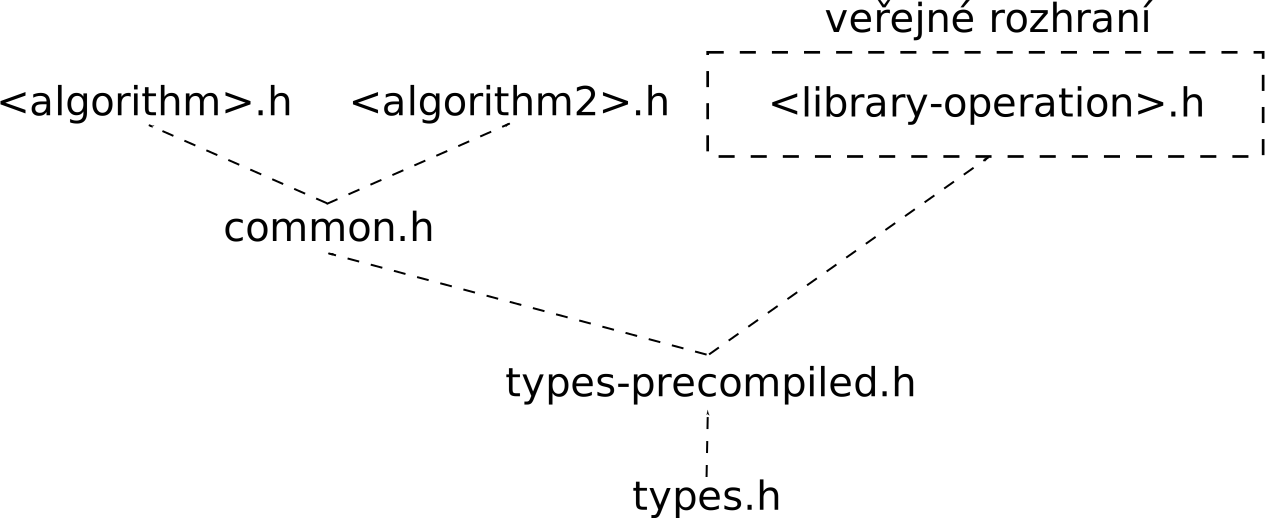
\includegraphics[scale=.25]{fig/header-dependencies.pdf}
	\caption{Diagram závislostí hlavičkových souborů}
\end{figure}\label{fig:header-dependecies}

hlavičkové soubory jsou rozděleny na veřejné a privátní rozhraní, kde privátní rozhraní je používáno pouze uvnitř knihovny. Hierarchickou strukturu je možné vidět na obrázku \ref{fig:header-dependecies}.

Jako výchozí hlavičkový soubor je použit types.h, který obsahuje definice datových struktur pro všechny algoritmy v podknihovně, které musí být viditelné i z veřejného rozhraní. Dalším souborem je types-precompiled.h, který je generován z types.h při překladu když se vybírá používaný algoritmus. common.h je hlavičkový soubor společný pro všechny algoritmy v podknihovně a algortihm.h pak obsahuje deklarace právě pro jeden konkrétní algoritmus.
sublib.h je pak hlavičkový soubor, který tvoří veřejné rozhraní ke knihovním funkcím.

Přesnou specifikaci rozhraní je možné nalézt v přiloženém CD ve složce \texttt{/lib/src/regex/regex.h}

\section{Použití knihovny}
Celou knihovnu je možné sestavit příkazem \texttt{make all} v hlavním adresáři knihovny.
Při tomto příkazu bude celá knihovna sestavena s definovaným NDEBUG, což má za následek vypuštění všech
volání funkce assert, která slouží pro ověřovaní správné funkčnosti.

Dalšími cíly pro program \texttt{make} jsou

\begin{itemize}
	\item{\texttt{test} - spustí automatické testování všech částí knihovny}
	\item{\texttt{bech} - spustí benchmarky všech částí knihovny}
	\item{\texttt{doc} - vygeneruje programovou dokumentaci ke všem částem knihovny}
	\item{\texttt{clean} - smaže všechny soubory vytvořené překladem}
\end{itemize}

\section{Rošíření knihovny}

Pro rozšíření knihovny je nutné přidat knihovnu implementující danou operaci
do adresáře \texttt{lib/src} a upravit příslušný soubor \texttt{Makefile} v daném adresáři.
Dále je vhodné vytvořit testovací program a sadu testů, kterou je možné automatizovaně spouštět a vyhodnocovat.
Tyto soubory pak umístit do adresáře \texttt{lib/test/<operace>}.
Další vhodnou součástí knihovny operace je benchmark pro vyhodnocení rychlosti/paměťové náročnosti jednotlivých
implementací dané operace.

\subsection{Packer header extraction}
V knihovně je již navrženo API pro operaci extrakci informací z hlaviček paketů.

\texttt{pc\_set} je struktura typu union, kde jsou všechny položky uloženy na stejném paměťovém místě
a jejich interpretace je odvozená dle typu položky, ke které je přistoupeno.

\begin{Verbatim}[commandchars=\\\{\}]
\PY{k}{typedef} \PY{k}{union}
\PY{p}{\PYZob{}}
	\PY{k+kt}{uint32\PYZus{}t} \PY{n}{number}\PY{p}{;}
	\PY{k+kt}{uint16\PYZus{}t} \PY{n}{number16}\PY{p}{;}
	\PY{k+kt}{char} \PY{n}{character}\PY{p}{;}
	\PY{n}{in\PYZus{}addr} \PY{n}{addr}\PY{p}{;}
\PY{p}{\PYZcb{}} \PY{n}{phe\PYZus{}item}\PY{p}{;}

\PY{k}{typedef} \PY{k}{union}
\PY{p}{\PYZob{}}
	\PY{k+kt}{uint32\PYZus{}t} \PY{n}{number}\PY{p}{;}
	\PY{k+kt}{uint16\PYZus{}t} \PY{n}{number16}\PY{p}{;}
	\PY{k+kt}{char} \PY{n}{character}\PY{p}{;}
	\PY{n}{in6\PYZus{}addr} \PY{n}{addr}\PY{p}{;}
\PY{p}{\PYZcb{}} \PY{n}{phe6\PYZus{}item}\PY{p}{;}

\PY{k+kt}{\PYZus{}Bool} \PY{n+nf}{phe\PYZus{}get}\PY{p}{(}\PY{k+kt}{char} \PY{o}{*} \PY{n}{input}\PY{p}{,} \PY{n}{phe\PYZus{}item} \PY{o}{*} \PY{n}{items}\PY{p}{,} \PY{p}{.}\PY{p}{.}\PY{p}{.}\PY{p}{)}\PY{p}{;}
\PY{k+kt}{\PYZus{}Bool} \PY{n+nf}{phe6\PYZus{}get}\PY{p}{(}\PY{k+kt}{char} \PY{o}{*} \PY{n}{input}\PY{p}{,} \PY{n}{phe6\PYZus{}item} \PY{o}{*} \PY{n}{items}\PY{p}{,} \PY{p}{.}\PY{p}{.}\PY{p}{.}\PY{p}{)}\PY{p}{;}
\end{Verbatim}


\subsection{Packer clasification}
V knihovně je již navrženo API pro operaci klasifikace paketů.

\begin{Verbatim}[commandchars=\\\{\}]
\PY{k}{typedef} \PY{k}{struct}
\PY{p}{\PYZob{}}
	\PY{k+kt}{unsigned} \PY{n}{rule}\PY{p}{;}
	\PY{k}{struct} \PY{n}{in\PYZus{}addr} \PY{n}{dst}\PY{p}{;}
	\PY{k}{struct} \PY{n}{in\PYZus{}addr} \PY{n}{src}\PY{p}{;}
	\PY{k+kt}{\PYZus{}Bool} \PY{n}{protocol}\PY{p}{;}
	\PY{k+kt}{short} \PY{n}{port}\PY{p}{;}
\PY{p}{\PYZcb{}} \PY{n}{pc\PYZus{}set}\PY{p}{;}

\PY{k}{typedef} \PY{k+kt}{void} \PY{n}{pc\PYZus{}root}\PY{p}{;}

\PY{n}{pc\PYZus{}root} \PY{o}{*} \PY{n+nf}{pc\PYZus{}init}\PY{p}{(}\PY{p}{)}\PY{p}{;}
\PY{k+kt}{void} \PY{n+nf}{pc\PYZus{}destroy}\PY{p}{(}\PY{n}{pc\PYZus{}root} \PY{o}{*} \PY{n}{root}\PY{p}{)}\PY{p}{;}
\PY{k+kt}{\PYZus{}Bool} \PY{n+nf}{pc\PYZus{}add}\PY{p}{(}\PY{n}{pc\PYZus{}root} \PY{o}{*} \PY{n}{root}\PY{p}{,} \PY{n}{pc\PYZus{}set} \PY{n}{set}\PY{p}{[}\PY{p}{]}\PY{p}{,} \PY{k+kt}{unsigned} \PY{n}{count}\PY{p}{)}\PY{p}{;}
\PY{k+kt}{\PYZus{}Bool} \PY{n+nf}{pc\PYZus{}update}\PY{p}{(}\PY{n}{pc\PYZus{}root} \PY{o}{*} \PY{n}{root}\PY{p}{,} \PY{n}{pc\PYZus{}set} \PY{n}{old}\PY{p}{,} \PY{n}{pc\PYZus{}set} \PY{n}{new}\PY{p}{)}\PY{p}{;}
\PY{k+kt}{void} \PY{n+nf}{pc\PYZus{}remove}\PY{p}{(}\PY{n}{pc\PYZus{}root} \PY{o}{*} \PY{n}{root}\PY{p}{,} \PY{n}{pc\PYZus{}set} \PY{n}{set}\PY{p}{)}\PY{p}{;}
\end{Verbatim}



\chapter{Výsledky}\label{chapter:results}
Tato kapitula shrnuje a vizualizuje dosažené výsledky při implementaci jednotlivých knihoven.
Benchmarky pro architekturu Intel proběhly na operačním systému Archlinux \footnote{https://www.archlinux.org/} s procesorem Intel(R) Core(TM) i3-2310M CPU @ 2.10GHz.

\section{Hledání nejdelšího shodného prefixu}

Hledání nejdelšího shodného prefixu bylo testováno na celkem pěti vstupních sadách dat, které
byly převzaty z volně dostupných dat RIPE\footnote{https://www.ripe.net/}.
Informace o testovaných sadách dat jsou zobrazeny v tabulce \ref{tab:lpm-input}.

\begin{table}[!htb]
	\center
	\label{tab:lpm-input}
	\caption{Informace v routovací tabulce pro benchmarky}
    \begin{tabular}{|l|l|l|l|}
    \hline
    Počet adres & Nejkratší prefix & Nejdelší prefix & Verze IP \\ \hline
    $1000$ & 13 & 31 & IPv4 \\ \hline
    $10000$ & 8 & 32 & IPv4 \\ \hline
    $100000$ & 8 & 32 & IPv4 \\ \hline
    $1000$ & 23 & 128 & IPv6 \\ \hline
    $10000$ & 19 & 128 & IPv6 \\ \hline
    \end{tabular}
\end{table}

Důvod proč není benchmark pro IPv6 se 100 000 záznamy ve směrovací tabulce je ten, že se mi nepovedlo
sehnat směrovací tabulku takové velikosti, což vzhledem k menší rozšířenosti IPv6 dává smysl.

Vyhledávání pak bylo testováno oproti sadě velikost $1000$ odpovídající verze IP, která je podmnožnou každé
rozsáhlejší sady dat.

Testováno bylo jak TreeBitmap ve všech variantách velikosti střídy, tedy $1-8$.
Jak je vidět na následujících grafech, tak nejlepších výsledků bylo dosaženo pro TreeBitmap s velkostí
střidy nastavenou na $5$ bitů a to jak pro IPv4 tak i pro IPv6.

Pro testování algoritmu Binary search on prefix length byla zvolena velikost hešovací tabulky
stejná jako velikost směrovacích dat. Tento přístup byl zvolen z důvodu významného vlivu
veliskosti hešovací tabulky na rychlost samotného vyhledávání. V nejhorším případě, tedy při
velikosti hešovací tabulky $100$ byl algortimus pomalejší pro hledání v tabulce se $100 000$ záznamy pomalejší
$400\times$.
U algoritmu bspl je doba vyhledání prefixu velice závislá na velikosti hešovací tabulky a proto je vhodné odhadnout počet záznamů tabulky alespoň řádově a dle toho pak nastavit velikost konstantu {\tt \_HTABLE\_SIZE} v souboru bspl.h na hodnotu, která alespoň řádově odpovídá předpodkládané velikosti hešovací tabulky.

Dalším důležitým faktorem pro efektivnost implementace je velikost datových struktur, která je znázroněna v následující tabulce.

\begin{table}[!htb]
	\center
	\label{tab:lpm-input}
	\caption{Velikosti datových struktur pro TreeBitmap}
    \begin{tabular}{|l|l|l|l|}
    \hline
    Velikost střídy & počet bytů \\ \hline
    1 & 24 \\ \hline
    2 & 24 \\ \hline
    3 & 24 \\ \hline
    4 & 24 \\ \hline
    5 & 32 \\ \hline
    6 & 40 \\ \hline
    7 & 64 \\ \hline
    8 & 112 \\ \hline
    \end{tabular}
\end{table}

Pro Binary search on prefix length pak bude velikost jednoho prvku stromu činit $48B$.
Pokud by došlo k rozdělení datových struktur pro jednotlivé verze IP protokolu
tak verze pro IPv4 by měla velikost $36B$.

Jak je vidět ve výše uvedené tabulce tak i přestože nejrychlejší implementací je TreeBitmap s střídou 5,
tak v případě omezené paměti by bylo vhodnější zvolit kompromis mezi rychlostí a paměťovou náročností v podobě
TreeBitmap s velikostí střídy 4. Dalším ovlivňujícím faktorem je odhadovaný počet záznamů směrovací tabulky, protože
nejrychlejší TBM-5 při existenci všech struktur na všech úrovních bude činit rozdíl zabraného místa oproti TBM4
celých $TODO dopočítat KB$, což je v kontextu FPGA případně ASIC implementace nezanedbatelné množství.

Také je důležité zmínit že z počtu očekávaných vstupních pravidel má také vliv na velikost struktury.
Do 256 záznamů zabírá pravidlo pouze 1byte, do 65536 záznamů pak 2 byty a pro více než 65536 pak celé čtyři byty pro uložení právě jednoho pravidla. Při uložení $65536$ adres to bude rozdíl mezi uložením $65537$ bude rozdíl činit
$200KB$

\begin{figure}[!htb]
	\centering
	\includegraphics[scale=1]{fig/lpm-ipv4.pdf}
	\caption{Benchmark pro IPv4}
\end{figure}\label{fig:lpm-ipv4}

\begin{figure}[!htb]
	\centering
	\includegraphics[scale=1]{fig/lpm-ipv6.pdf}
	\caption{Benchmark pro IPv6}
\end{figure}\label{fig:lpm-ipv4}

\section{Hledání řetězců}

\begin{figure}[!htb]
	\centering
	\includegraphics[scale=0.7]{fig/pm.pdf}
	\caption{Benchmark pro knihovnu pm}
\end{figure}\label{fig:pm}

\section{Hledání regulárních výrazů}

\begin{figure}[!htb]
	\centering
	\includegraphics[scale=0.7]{fig/regex.pdf}
	\caption{Benchmark pro knihovnu regex}
\end{figure}\label{fig:regex}

\chapter{Závěr}\label{chapter:conclusion}
Cílem této práce bylo popsat a navrhnout aplikační programové rozhraní časově kritické operace v oblasti počítačových sítí,
konkrétně vyhledání nejdelšího shodného prefixu za využití algoritmů Binary search on prefix length
a TreeBitmap. Operace používané na směrovačích pro zjištění jakou cestou směrovat přicházející pakety.
Dalšími operacemi jsou hledání řetězců a hledání regulárních výrazů v paketech a jejich datech.
Pro operaci hledání řetězců je to konkrétně algoritmus Aho-Corasick \cite{aho} umožňují v
při jednom průchodu vstupními daty vyhodnit zda se v datech nacházejí specifikovaná klíčová slova
a poté hledání regulárních výrazů. Obě zmíněné operace jsou používané v paketových filtrech,
které tvoří jádro systémů pro detekci útoků (IDS) a prevenci útoků (IPS). Do skupiny těchto
systémů patří firewally jak softwarové tak hardwarové. Mezi další operace operace pak patří
analýza a extrakce hlaviček paketů a obecná klasifikace paketů.

Dále je to pak implementace operací hledání nejdelšího shodného prefixu, hledání řetězců
a hledání regulárních výrazů. Při implementaci bylo dosaženo rychlosti zpracování N paketů za sekundu
při velikosti $100000$ záznamů routovací tabulky pro IP adresy verze 4 a N paketů/sekunda při velikosti
routovací tabulky $10000$ pro IP adresy verze 6. Pro operaci hledání podřetězců bylo
do dosaženo rychlosti zpracování N paketů za sekundu v závislosti na počtu shodných písmen
při lineární náročnosti v závislosti na velikost dat v paketech. Experimentování bylo prováděno
na vzorku dat odchycených ze standardního síťového provozu jednoho osobního počítače. Jako vzorek
testovaných klíčových slov bylo využito klíčových definovaných pro HTTP\footnote{Hyper-text transfer protocol}.
Pří experimentování s regulárními výrazy byly jako vstupní data použita stejná data jako pro hledání řetězců,
ale jako regulární výraz byly použity matchování URL\footnote{Uniform resource locator} adres.

Část této práce pojednávající o hledání nejdelšího shodného prefixu vychází z publikací
\cite{tbm}, \cite{bspl}, a dalších. Hledání řetězců vychází z \cite{aho} a hledání regilárních výrazů
 z \cite{}.

\section{Další rozšíření}
Jako kroky navazující na tuto práci je možné implementovat zbývající operace, které implemetnovány nebyly.
Těmito operacemi je klasifikace paketů a analýza a extrakce hlaviček paketů.

\subsection{Optimalizace}
U implementace \texttt{Binary search on prefix length} je možné rozdělit strukturu \texttt{\_bspl\_node}
na dvě a to jednu pro každou verzi IP protokolu. Tím se dosáhne snížení paměťové náročnosti
pro implementaci IPv4 o 12B pro každý uzel. To s sebou nese nutnost upravit všechny funkce pracující
s položkou \texttt{prefix} v rámci této struktury.

Další optimalizací je přepsání leaf-pushing do iterativní průchod za použití Morrisova algoritmu \cite{morris},
který umožňuje průchod stromovou strukturou bez použití rekurze a zásobníku.

Dále je možné spojit položky \texttt{type} a \texttt{prefix\_length} struktury \texttt{\_bspl\_node}
do jednoho byte. To je možné z důvodu rozsahu \texttt{prefix\_length} $1-128$ a pouze dvou typů uzlu,
což je možné reprezentovat jedním bytem.

\subsection{Stress-testing}
Ze specifikace požadavků na implementaci knihovny v nízkoúrovňovém jazyce C je zřejmé,
že knihovna bude používána i na vestavěných systémech disponujících omezenou pamětí a z toho
důvodu by jedním z dalších kroků mohlo být formální testování s nedostatkem paměti.
To by mohlo dát rozsahem na celou další práci. Je nutné ověřit, že knihovna bude
reagovat správným způsob a nezpůsobí pád systému v rámci kterého je spouštěna.
